\documentclass[a4paper,12pt]{article}

\usepackage{a4wide}
\usepackage{amsfonts}
\usepackage{amsmath}
\usepackage{amssymb}
\usepackage{csquotes}
\usepackage{lipsum}
\usepackage{bm}
\usepackage{tabularx}
\usepackage{longtable}

\usepackage{graphicx}  % For including images
\usepackage{xcolor}  % For a colorfull presentation
\usepackage{listings}  % For presenting code 

\usepackage{algorithm}
\usepackage[noend]{algpseudocode}
\makeatletter
\def\BState{\State\hskip-\ALG@thistlm}
\makeatletter
\usepackage[normalem]{ulem}
\usepackage{array}
\usepackage{hyperref}
% \usepackage[hyphens]{url}

\hypersetup{
  colorlinks=true,
  linkcolor=blue,
  urlcolor=blue,
  citecolor=blue
}
\newcommand{\bluehref}[2]{\href{#1}{\textcolor{blue}{\uline{#2}}}}
\makeatletter
\newcommand*{\citelinktext}[2]{%
  \hyper@@link[cite]{}{cite.#1}{#2}}
\makeatother

\usepackage{booktabs} 
\usepackage{enumitem}
\usepackage{bbm}
\usepackage{tcolorbox}

\usepackage{minted}
\usepackage{subcaption}

\usepackage[font=small,labelfont=bf]{caption}

\usepackage{fullpage,amsmath,amsthm,amssymb}
\newtheorem*{solution}{Solution}
\newtheorem*{part1}{Part 1}
\newtheorem*{part2}{Part 2}

\newcommand{\Cov}{\mathrm{Cov}}
\newcommand{\Var}{\mathrm{Var}}
\newcommand{\rank}{\mathrm{rank}}
\newcommand{\Span}{\mathrm{span}}
\newcommand{\clip}{\mathrm{clip}}
\newcommand{\Dim}{\mathrm{dim}}

\newcolumntype{Y}{>{\raggedright\arraybackslash}X}

\tcbset{
  colback=gray!3,
  colframe=black!20,
  boxsep=1mm,
  left=1mm,
  right=1mm,
  top=1mm,
  bottom=1mm,
}

\usepackage{changepage}
\newenvironment{restoretext}%
    {
     \begin{adjustwidth}{}{\leftmargin}%
    }{\end{adjustwidth}
     }

% Definition of a style for code, matter of taste
\lstdefinestyle{mystyle}{
  language=Python,
  basicstyle=\ttfamily\footnotesize,
  backgroundcolor=\color[HTML]{F7F7F7},
  rulecolor=\color[HTML]{EEEEEE},
  identifierstyle=\color[HTML]{24292E},
  emphstyle=\color[HTML]{005CC5},
  keywordstyle=\color[HTML]{D73A49},
  commentstyle=\color[HTML]{6A737D},
  stringstyle=\color[HTML]{032F62},
  emph={@property,self,range,True,False},
  morekeywords={super,with,as,lambda},
  literate=%
    {+}{{{\color[HTML]{D73A49}+}}}1
    {-}{{{\color[HTML]{D73A49}-}}}1
    {*}{{{\color[HTML]{D73A49}*}}}1
    {/}{{{\color[HTML]{D73A49}/}}}1
    {=}{{{\color[HTML]{D73A49}=}}}1
    {/=}{{{\color[HTML]{D73A49}=}}}1,
  breakatwhitespace=false,
  breaklines=true,
  captionpos=b,
  keepspaces=true,
  numbers=none,
  showspaces=false,
  showstringspaces=false,
  showtabs=false,
  tabsize=4,
  frame=single,
}
\lstset{style=mystyle}

\begin{document}
\begin{titlepage}
    \centering
    \vspace*{1cm}
    
    \Huge
    \textbf{CSC490: Assignment 2}
    
    \vspace{0.5cm}
    
    \vspace{1.5cm}
    
    \textbf{Team Members}
    
    \vspace{0.8cm}
    
    \large
    \begin{tabular}{ll}
        \textbf{Name} & \textbf{Student ID} \\
        \midrule
        Aarya Prakash & 1008790257 \\
        Derek Huynh & 1008849052 \\
        Merrick Liu & 1008951920 \\
        Rhys Balevicius & 1000801974 \\
    \end{tabular}
    
    \vfill
    
    \large
    University of Toronto\\
    Department of Computer Science    
\end{titlepage}

% \title{CSC490 ML Engineering Capstone (2026)\\Assignment 1}
% \author{\color{red}Rhys Balevicius, Merrick Liu, Aarya Prakash, Derek Huynh}
% \title{}
% \date{}
% \maketitle

% \tableofcontents % Generates the table of contents
% \newpage % Start a new page after the table of contents

% ================================================================================================
%
%
%
%
%
% ================================================================================================


\section{Aspirational Datasets}

% Imagine you had a magic wand, what datasets would your team need to be successful in this project? Create an aspirational list of datasets with the data schemas you would like.

Our goal is to improve the efficacy of AI coding agents, which may produce incorrect changes because they lack relevant context that exists outside their immediate working scope. To build and evaluate systems that surface this missing context, the ideal dataset would consist of tuples pairing a coding task with a point-in-time snapshot of the full software environment: the target repository, its transitive dependencies, documentation, and version history along with a gold label identifying the precise, minimal set of non-local information an agent would have needed to produce a correct change. This label is the core artifact: it answers the question \textit{"what did the agent need to know, but didn't, in order to get this right?"} and it spans multiple axes of context, including interface contracts and type signatures across module and library boundaries, downstream callers and invariants that a local change might violate, architectural conventions and design rationale recoverable from project history, and relevant documentation or specifications from external dependencies.\\

\noindent Each entry would additionally include a failed agent attempt (produced without sufficient context), the corresponding corrected code (produced by a human or by an agent given adequate context), and the failure signal linking the two such as a test failure, type error, or behavioural regression. The causal structure of this data is what makes it powerful: the delta between the failed and successful attempts is attributable to the presence or absence of the labelled context. With such a dataset, one could train and evaluate any retrieval or reasoning approach against a ground-truth definition of what "the right context" is for a given task, and measure whether surfacing it actually changes agent outcomes.\\

\noindent Note: nested type definitions are provided in Appendix~\ref{app:typedefs}.

\subsection*{Aspirational Dataset 1: Context-Attributed Agent Failures}

\noindent Each row captures a coding task where an agent failed, the corrected outcome, and a precise attribution of what non-local context was missing. 

\begin{tcolorbox}[title=Task]
\footnotesize
\begin{tabularx}{\linewidth}{@{} l l Y @{}}
\toprule
\textbf{Field} & \textbf{Type} & \textbf{Notes} \\
\midrule
repo & \texttt{str} & Target repository \\
repo\_snapshot & \texttt{commit\_sha} & Frozen state of repo at task time \\
dependency\_snapshot & \texttt{[package@version]} & Pinned versions of all transitive dependencies \\
task & \texttt{str} & Natural language description of the coding task \\
agent\_attempt & \texttt{AgentAttempt} & Incorrect attempt record \\
failure\_signal & \texttt{FailureSignal} & Failure manifestation \\
corrected\_diff & \texttt{Diff} & Correct change \\
missing\_context & \texttt{[MissingContext]} & Required unseen context \\
\bottomrule
\end{tabularx}
\end{tcolorbox}

% ================================================================================================
\subsection*{Aspirational Dataset 2: Interface Contracts and Cross-Boundary Specifications}

\noindent Each row describes a function or module boundary, its (possibly implicit) contract, and the set of callers/consumers that depend on that contract across repo and library boundaries.

\begin{tcolorbox}[title=Function]
\footnotesize
\begin{tabularx}{\linewidth}{@{} l l Y @{}}
\toprule
\textbf{Field} & \textbf{Type} & \textbf{Notes} \\
\midrule
repo & \texttt{str} & Repository \\
repo\_snapshot & \texttt{commit\_sha} & Frozen state \\
function & \texttt{fully\_qualified\_name} & Canonical name \\
defined\_in & \texttt{\{file, span\}} & Definition location \\
contract & \texttt{Contract} & Behavioural specification \\
consumers & \texttt{[Consumer]} & Call sites \\
known\_violations & \texttt{[KnownViolation]} & Historical breaks \\
\bottomrule
\end{tabularx}
\end{tcolorbox}

% ================================================================================================
\subsection*{Aspirational Dataset 3: Downstream Impact Chains}

\noindent Each row captures a local change and the full causal chain through which it produces a failure at a distant location.

\begin{tcolorbox}[title=ChangeImpact]
\footnotesize
\begin{tabularx}{\linewidth}{@{} l l Y @{}}
\toprule
\textbf{Field} & \textbf{Type} & \textbf{Notes} \\
\midrule
repo & \texttt{str} & Repository \\
repo\_snapshot & \texttt{commit\_sha} & Frozen state \\
local\_change & \texttt{Diff} & Triggering modification \\
change\_location & \texttt{\{file, function\}} & Origin of change \\
failure\_location & \texttt{\{file, function, test\}} & Where breakage surfaced \\
causal\_chain & \texttt{[CausalNode]} & Propagation path \\
chain\_length & \texttt{int} & Hop count \\
minimal\_context & \texttt{[\{file, span\}]} & Minimal foresight set \\
\bottomrule
\end{tabularx}
\end{tcolorbox}

% ================================================================================================
\newpage
\subsection*{Aspirational Dataset 4: Architectural Conventions and Project Norms}

\noindent Each row encodes an implicit or explicit convention in a codebase, examples of code that follow it, and examples of agent-generated code that violates it.

\begin{tcolorbox}[title=ConventionSchema]
\footnotesize
\begin{tabularx}{\linewidth}{@{} l l Y @{}}
\toprule
\textbf{Field} & \textbf{Type} & \textbf{Notes} \\
\midrule
repo & \texttt{str} & Repository \\
repo\_snapshot & \texttt{commit\_sha} & Frozen state \\
convention & \texttt{Convention} & Normative pattern \\
conforming\_examples & \texttt{[\{file, span\}]} & Correct usages \\
violations & \texttt{[Violation]} & Broken instances \\
\bottomrule
\end{tabularx}
\end{tcolorbox}

% ================================================================================================
\subsection*{Aspirational Dataset 5: Design Rationale and Temporal Context}

\noindent Each row links a region of code to the historical decisions that explain \textit{why} it is the way it is: the context an agent needs to avoid "cleaning up" intentional complexity.

\begin{tcolorbox}[title=CodeHistory]
\footnotesize
\begin{tabularx}{\linewidth}{@{} l l Y @{}}
\toprule
\textbf{Field} & \textbf{Type} & \textbf{Notes} \\
\midrule
repo & \texttt{str} & Repository \\
repo\_snapshot & \texttt{commit\_sha} & Frozen state \\
code\_region & \texttt{\{file, span\}} & Location \\
current\_form & \texttt{str} & Present code \\
history & \texttt{[HistoryEntry]} & Prior commits \\
rationale & \texttt{Rationale} & Design justification \\
naive\_refactors & \texttt{[NaiveRefactor]} & Tempting but incorrect changes \\
\bottomrule
\end{tabularx}
\end{tcolorbox}

% ================================================================================================
\subsection*{Aspirational Dataset 6: Cross-Repository Dependency Context}

\noindent Each row captures a usage of an external library and the external documentation, source, or changelog context needed to use it correctly.

\begin{tcolorbox}[title=DependencyUsage]
\footnotesize
\begin{tabularx}{\linewidth}{@{} l l Y @{}}
\toprule
\textbf{Field} & \textbf{Type} & \textbf{Notes} \\
\midrule
consumer\_repo & \texttt{str} & Consuming repo \\
repo\_snapshot & \texttt{commit\_sha} & Frozen state \\
dependency & \texttt{\{name, version\}} & External package \\
usage\_location & \texttt{\{file, span\}} & Call site \\
api\_used & \texttt{fully\_qualified\_name} & Referenced symbol \\
required\_context & \texttt{[RequiredContext]} & External knowledge \\
version\_sensitivity & \texttt{VersionSensitivity} & Version constraints \\
misuse\_examples & \texttt{[MisuseExample]} & Incorrect usages \\
\bottomrule
\end{tabularx}
\end{tcolorbox}

% ================================================================================================
%
%
%
%
%
% ================================================================================================
\newpage
\section{Reality Check}

% Now review which datasets are actually available. Create a table of datasets that you could use for your project. Include public datasets, data you can scrape or data you can generate. For each dataset include a link to the source, a description of the data and commentary on why it is relevant to your project.

The ideal schema above asks for five things per task: a task statement, a point-in-time code/dependency snapshot, a failure signal, a corrected change, and explicit attribution of the missing non-local context. No single public source gives all five, so the practical path is to combine (1) existing benchmarks, (2) mined web data, and (3) synthetic generation pipelines.

\footnotesize
\begin{longtable}{@{} p{3cm} p{5cm} p{7cm} @{}}
% \begin{longtable}{@{} l L{3.2cm} L{5.2cm} L{5.2cm} @{}}

\toprule
\textbf{Dataset} & \textbf{Description} & \textbf{Commentary} \\
\midrule
\endfirsthead

\toprule
\textbf{Dataset} & \textbf{Description} & \textbf{Commentary} \\
\midrule
\endhead

\bottomrule
\endfoot

\href{https://www.swebench.com/original.html}{SWE-bench} &
2,294 task instances from 12 Python repos. Each instance includes issue, PR, and test patch. &
\textbf{Primary evaluation benchmark.} Run agents with/without MCP service and measure resolution-rate delta. \\

\href{https://huggingface.co/datasets/SWE-bench-Live/SWE-bench-Live}{SWE-bench-Live} &
Continuously updated variant of SWE-bench with more recent issues post-training-cutoff. Same schema (issue, PR, test patch). &
\textbf{Anti-contamination eval set.} Prevents inflated scores from benchmark leakage into foundation model training data. Use as a held-out evaluation set once our system is tuned on original SWE-bench. \\

\href{https://github.com/SWE-bench/SWE-smith}{SWE-smith} &
Toolkit for generating synthetic SWE-bench-style instances via automated code transformations (bug injection, context removal). Can produce instances at scale on arbitrary repos. &
\textbf{Scale up evaluation + training data.} Original SWE-bench is only 2K instances; SWE-smith enables orders-of-magnitude more. Useful for stress-testing retrieval across diverse repo structures and for generating Dataset~1 (context-attributed failures) synthetically with known ground-truth context. \\

\href{https://huggingface.co/datasets/SWE-Gym/SWE-Gym-Raw}{SWE-Gym-Raw} &
Execution environments for SWE-bench instances. Provides Docker setups with pinned dependencies for running tests against agent patches. &
\textbf{Evaluation infrastructure (not a dataset).} Enables reproducible eval harness execution and avoids building custom sandboxes. Low priority for data ingestion; high priority for evaluation. \\

\href{https://huggingface.co/datasets/nebius/SWE-rebench-leaderboard}{SWE-rebench} &
Re-evaluated SWE-bench leaderboard with stricter pass/fail criteria (avoids false positives from flaky tests, overcounting, etc.). &
\textbf{Meta-resource for evaluation calibration.} Not a dataset to ingest. Use their methodology to ensure our eval harness produces trustworthy results. Reference only. \\

\href{https://github.com/Leolty/repobench}{RepoBench} &
Benchmark for repo-level code completion. Tasks require cross-file context (imports, related functions in other files) to complete a function body correctly. 11K instances across Python and Java. &
\textbf{Directly relevant for code graph retrieval evaluation.} Tests whether the system surfaces correct cross-file context (e.g., \texttt{get\_callers}, \texttt{get\_contract}). Strong eval set for the indexing layer independent of the full MCP pipeline. Covers Dataset~2 (contracts/cross-boundary specs). \\

\href{https://huggingface.co/datasets/bigcode/the-stack-v2}{The Stack v2} &
67.5~TB of permissively licensed source code from Software Heritage, spanning hundreds of languages. &
\textbf{Training resource for embeddings (not an eval dataset).} Suitable for training or fine-tuning code embeddings (e.g., Milvus semantic search). Also useful for large-scale convention mining (Dataset~4). Heavy to process; use targeted subsets. \\

\href{https://docs.softwareheritage.org/devel/swh-export/graph/}{Software Heritage Graph} &
Complete graph of publicly known software development: repos, commits, directories, files, and their relationships. Available as node+edge export. &
\textbf{Dependency and impact analysis at scale.} Can support Dataset~3 (downstream impact chains) and Dataset~6 (cross-repo dependency context) via ecosystem-level call/import graphs. Very heavy; best used via targeted API or BigQuery queries rather than full ingestion. \\

\href{https://www.gharchive.org/}{GH Archive} &
Complete GitHub event stream since 2011 (PushEvents, PullRequestEvents, IssuesEvents, IssueCommentEvents, etc.), available as JSON via BigQuery or direct download. &
\textbf{Primary scraped training source.} Mine issue$\rightarrow$PR$\rightarrow$fix chains at scale. Review comments often contain explicit missing-context signals (e.g., “this breaks because of X in module Y”). Feeds Datasets~1 and~5 (context-attributed failures, design rationale) and supports mental model construction via repo evolution. High priority for the offline pipeline. \\

\href{https://docs.deps.dev/bigquery/v1/}{deps.dev} &
Google's dataset of dependency relationships across package ecosystems (npm, PyPI, Go, Maven, Cargo, etc.), available via BigQuery. Includes dependency graphs, versions, advisories, and licenses. &
\textbf{Feeds \texttt{get\_dependency\_context} and Dataset~6.} Provides version graphs, breaking-change signals, and advisory data when indexing repo dependencies. High priority for the dependency index. \\

\href{https://github.com/github/CodeSearchNet}{CodeSearchNet} &
 code--docstring pairs across six languages (Python, Java, JS, PHP, Go, Ruby), originally released for training code search models. &
\textbf{Training data for embedding models.} Provides high-quality code+NL pairs for contrastive learning (e.g., Milvus semantic search). Also useful for evaluating NL$\rightarrow$code retrieval performance (e.g., \texttt{get\_context\_for\_change}). Medium priority. \\

Mutation-induced failing patches &
Generate via \texttt{mutmut} (or similar) on repos with tests. Inject mutations, run tests, retain failing mutants. Produces (\texttt{mutation\_diff}, \texttt{failing\_tests}, \texttt{original\_code}) triples. &
\textbf{High-volume source for Datasets~1 and~3.} Controlled perturbations provide exact change provenance and traceable failure paths. Suitable for large-scale retrieval-ranker training (“what context would have prevented this mistake?”). Generation should run on repos already in the data lake. \\

Mutation-repair pairs with context budgets &
For each mutated bug, collect an agent fix under limited context and under augmented context; compare outcomes. &
\textbf{Highest-value synthetic dataset.} Directly captures the causal signal: did context $X$ change the outcome from wrong to right? Provides ground truth for training the ranking in \texttt{get\_context\_for\_change}. Expensive to generate (requires agent runs), but highest signal-to-noise ratio. \\

Documentation generation &
Generate or extract docstrings and use them to train similarity between code semantics and natural language descriptions. &
\textbf{Secondary priority.} Supports embedding fine-tuning to better align code and documentation (e.g., Milvus). Improves \texttt{get\_dependency\_context} and other NL-based retrieval. Can be deferred until semantic search becomes the bottleneck. \\

\href{https://docs.github.com/en/graphql}{Closed issues + closing PRs + merge diffs} &
Mine via the GitHub GraphQL API: issue text, discussion threads, linked PRs, review comments, and commit diffs. Produces (\texttt{task\_description}, \texttt{discussion\_context}, \texttt{fix\_diff}) tuples. &
\textbf{Primary scraped dataset (high priority).} Closest approximation to naturally occurring Dataset~1 instances. Review comments often contain explicit missing-context annotations (“this breaks X because Y”). Feeds retrieval ranking, mental model construction, and convention mining. Should be prioritized in the offline pipeline. \\

\end{longtable}

% ================================================================================================
%
%
%
%
%
% ================================================================================================

\section{Data-processing pipelines}

% Design and implement a data processing pipeline for your project. This should include data ingestion, cleaning, transformation and data lake/warehouse design.

% Key Requirements:
% • Data schemas
% • Pipeline diagrams with the technologies you are using (open source frameworks are helpful) 
% • When the pipelines will run and for which use cases
% • Code for an initial version of this pipeline
% • Include next steps for features you did not implement in the writeup

The data-processing pipeline is implemented as the execution plane of Lighthouse and is designed to continuously supply high-quality context to the MCP service while also producing durable datasets for evaluation and model-improvement work. Architecturally, the pipeline runs as long-lived Temporal workers and applies a consistent stage model across online and offline workflows: ingest source data, clean and normalize it, transform it into retrieval/evaluation artifacts, and store outputs in a two-tier storage design. In this design, large raw and curated files are written to an S3-based data lake (bronze/silver/gold), while structured operational tables and queryable metadata are stored in Postgres. Retrieval-ready vectors are stored in Milvus.

\subsection{Data Schemas}

\noindent Lighthouse operates in two complementary pipeline modes. The online pipeline is request-driven and focuses on indexing freshness and low-latency readiness for MCP tool calls. The offline pipeline is schedule-driven and focuses on durable dataset curation for evaluation and retrieval-quality improvements: rolling scraped sources are ingested incrementally, synthetic datasets are refreshed on cadence, and version-pinned benchmark snapshots are treated as immutable to preserve reproducible baselines.

\subsubsection{Online indexing/control schemas}

\captionsetup{type=table}
\begin{tcolorbox}[title=IndexJobSchema]
\footnotesize
\begin{tabularx}{\linewidth}{@{} l l Y @{}}
\toprule
\textbf{Field} & \textbf{Type} & \textbf{Notes} \\
\midrule
job\_id & \texttt{str} & Unique indexing job identifier \\
workflow\_id & \texttt{str} & Temporal workflow identifier \\
repo\_id & \texttt{str} & Stable repository identifier \\
ref & \texttt{str} & Branch or tag context \\
status & \texttt{IndexStatus} & Job lifecycle state \\
stage & \texttt{IndexStage} & Current pipeline stage \\
progress\_pct & \texttt{int} & Progress percentage (0--100) \\
error\_code & \texttt{str | null} & Machine-readable failure code \\
error\_message & \texttt{str | null} & Human-readable failure message \\
created\_at & \texttt{timestamp} & Job creation time \\
updated\_at & \texttt{timestamp} & Last status update time \\
\bottomrule
\end{tabularx}
\end{tcolorbox}

\noindent \textit{Per-job execution progress, stage transitions, and failure details for runtime and offline indexing runs.}\\

\begin{tcolorbox}[title=IndexStateSchema]
\footnotesize
\begin{tabularx}{\linewidth}{@{} l l Y @{}}
\toprule
\textbf{Field} & \textbf{Type} & \textbf{Notes} \\
\midrule
repo\_id & \texttt{str} & Stable repository identifier \\
ref & \texttt{str} & Branch or tag context \\
snapshot\_sha & \texttt{commit\_sha} & Indexed commit represented by this state \\
status & \texttt{IndexStatus} & Readiness/freshness state \\
active\_job\_id & \texttt{str | null} & Current active job if indexing is in progress \\
stale\_after & \texttt{timestamp} & Freshness threshold for this index \\
last\_indexed\_at & \texttt{timestamp} & Last successful index completion \\
updated\_at & \texttt{timestamp} & Last state update time \\
\bottomrule
\end{tabularx}
\end{tcolorbox}

\noindent \textit{Represents the latest readiness and freshness state for each \texttt{(repo\_id, ref)} pair consumed by MCP.}

\subsubsection{Offline dataset schemas}

\begin{tcolorbox}[title=RepoSnapshotSchema]
\footnotesize
\begin{tabularx}{\linewidth}{@{} l l Y @{}}
\toprule
\textbf{Field} & \textbf{Type} & \textbf{Notes} \\
\midrule
repo\_id & \texttt{str} & Stable repository identifier \\
ref & \texttt{str} & Branch or tag context \\
snapshot\_sha & \texttt{commit\_sha} & Point-in-time repository snapshot \\
source & \texttt{str} & Upstream source name \\
captured\_at & \texttt{timestamp} & Ingestion timestamp \\
\bottomrule
\end{tabularx}
\end{tcolorbox}

\noindent \textit{Stores reproducible point-in-time repository snapshots used to anchor downstream dataset records.} \\

\begin{tcolorbox}[title=DatasetInstanceSchema]
\footnotesize
\begin{tabularx}{\linewidth}{@{} l l Y @{}}
\toprule
\textbf{Field} & \textbf{Type} & \textbf{Notes} \\
\midrule
instance\_id & \texttt{str} & Unique dataset instance identifier \\
task & \texttt{str} & Task/problem description \\
repo\_id & \texttt{str} & Repository identifier \\
snapshot\_sha & \texttt{commit\_sha} & Snapshot associated with this instance \\
failure\_type & \texttt{str} & Failure category label \\
failure\_ref & \texttt{str} & Pointer to failing output/signal \\
corrected\_diff\_ref & \texttt{str} & Pointer to corrected change artifact \\
split & \texttt{str} & Dataset split (train/validation/test) \\
created\_at & \texttt{timestamp} & Record creation time \\
\bottomrule
\end{tabularx}
\end{tcolorbox}

\noindent \textit{Defines the canonical task, failure, and fix record used for training and evaluation datasets.}\\ 

\begin{tcolorbox}[title=ContextLabelSchema]
\footnotesize
\begin{tabularx}{\linewidth}{@{} l l Y @{}}
\toprule
\textbf{Field} & \textbf{Type} & \textbf{Notes} \\
\midrule
instance\_id & \texttt{str} & Linked dataset instance \\
source\_type & \texttt{str} & Context origin (repo/dependency/doc/history) \\
location & \texttt{str} & File span, URL, or commit reference \\
context\_type & \texttt{str} & Context class (contract/caller/invariant/etc.) \\
relevance\_reason & \texttt{str} & Why this context matters \\
created\_at & \texttt{timestamp} & Record creation time \\
\bottomrule
\end{tabularx}
\end{tcolorbox}

\noindent \textit{Captures structured attribution of missing non-local context for each dataset instance.}\\

\begin{tcolorbox}[title=QualityMetricSchema]
\footnotesize
\begin{tabularx}{\linewidth}{@{} l l Y @{}}
\toprule
\textbf{Field} & \textbf{Type} & \textbf{Notes} \\
\midrule
run\_id & \texttt{str} & Linked pipeline run identifier \\
metric\_name & \texttt{str} & Metric key/name \\
metric\_value & \texttt{float} & Numeric metric value \\
metric\_context & \texttt{str} & Scope/context label for interpretation \\
measured\_at & \texttt{timestamp} & Measurement timestamp \\
\bottomrule
\end{tabularx}
\end{tcolorbox}

\noindent\textit{Stores quality and completeness metrics used to monitor dataset integrity and drift.}\\

\begin{tcolorbox}[title=PipelineRunSchema]
\footnotesize
\begin{tabularx}{\linewidth}{@{} l l Y @{}}
\toprule
\textbf{Field} & \textbf{Type} & \textbf{Notes} \\
\midrule
run\_id & \texttt{str} & Unique pipeline run identifier \\
workflow\_type & \texttt{str} & Workflow family (offline/runtime/mental-model) \\
source\_name & \texttt{str} & Dataset/source adapter name \\
status & \texttt{str} & Run lifecycle state \\
started\_at & \texttt{timestamp} & Run start time \\
finished\_at & \texttt{timestamp | null} & Run completion time \\
records\_in & \texttt{int} & Input row count \\
records\_out & \texttt{int} & Output row count \\
error\_code & \texttt{str | null} & Failure code if run did not succeed \\
\bottomrule
\end{tabularx}
\end{tcolorbox}

\noindent \textit{Provides run-level observability, auditability, and operational health tracking for pipeline executions.}

% ================================================================================================
\subsection{Pipelines}

\subsubsection{Schedules and Use Cases}

\begin{table}[H]
\centering
\footnotesize
\begin{tabular}{@{} >{\raggedright\arraybackslash}p{0.35\linewidth} >{\raggedright\arraybackslash}p{0.20\linewidth} >{\raggedright\arraybackslash}p{0.37\linewidth} @{}}
\toprule
\textbf{Pipeline} & \textbf{Schedule} & \textbf{Primary use case} \\
\midrule
Runtime indexing (\texttt{RuntimeIndexWorkflow}) & Event-driven (on MCP request) & Create or refresh repository context so MCP tool calls can return current results. \\
Offline benchmark snapshot ingestion (\texttt{OfflineDatasetWorkflow}) & Manual or on new benchmark release & Import and normalize immutable benchmark snapshots for reproducible baselines. \\
Evaluation refresh jobs & Monthly or on snapshot update & Recompute fail-to-pass delta and regression-rate trendlines over pinned benchmark data. \\
Offline rolling scraped ingestion (\texttt{OfflineDatasetWorkflow}) & Daily incremental & Ingest issue to PR to diff chains with append/upsert semantics for continuously updated training/eval slices. \\
Offline synthetic dataset refresh (\texttt{OfflineDatasetWorkflow}) & Weekly & Regenerate synthetic mutation-repair datasets and derived features with versioned generators. \\
Offline targeted reprocessing (\texttt{OfflineDatasetWorkflow}) & Event-driven/manual & Reprocess impacted partitions only after schema updates, transformation fixes, or data correction events. \\
\bottomrule
\end{tabular}
\end{table}

\subsubsection{Pipeline Diagrams}

\begin{figure}[H]
  \centering
  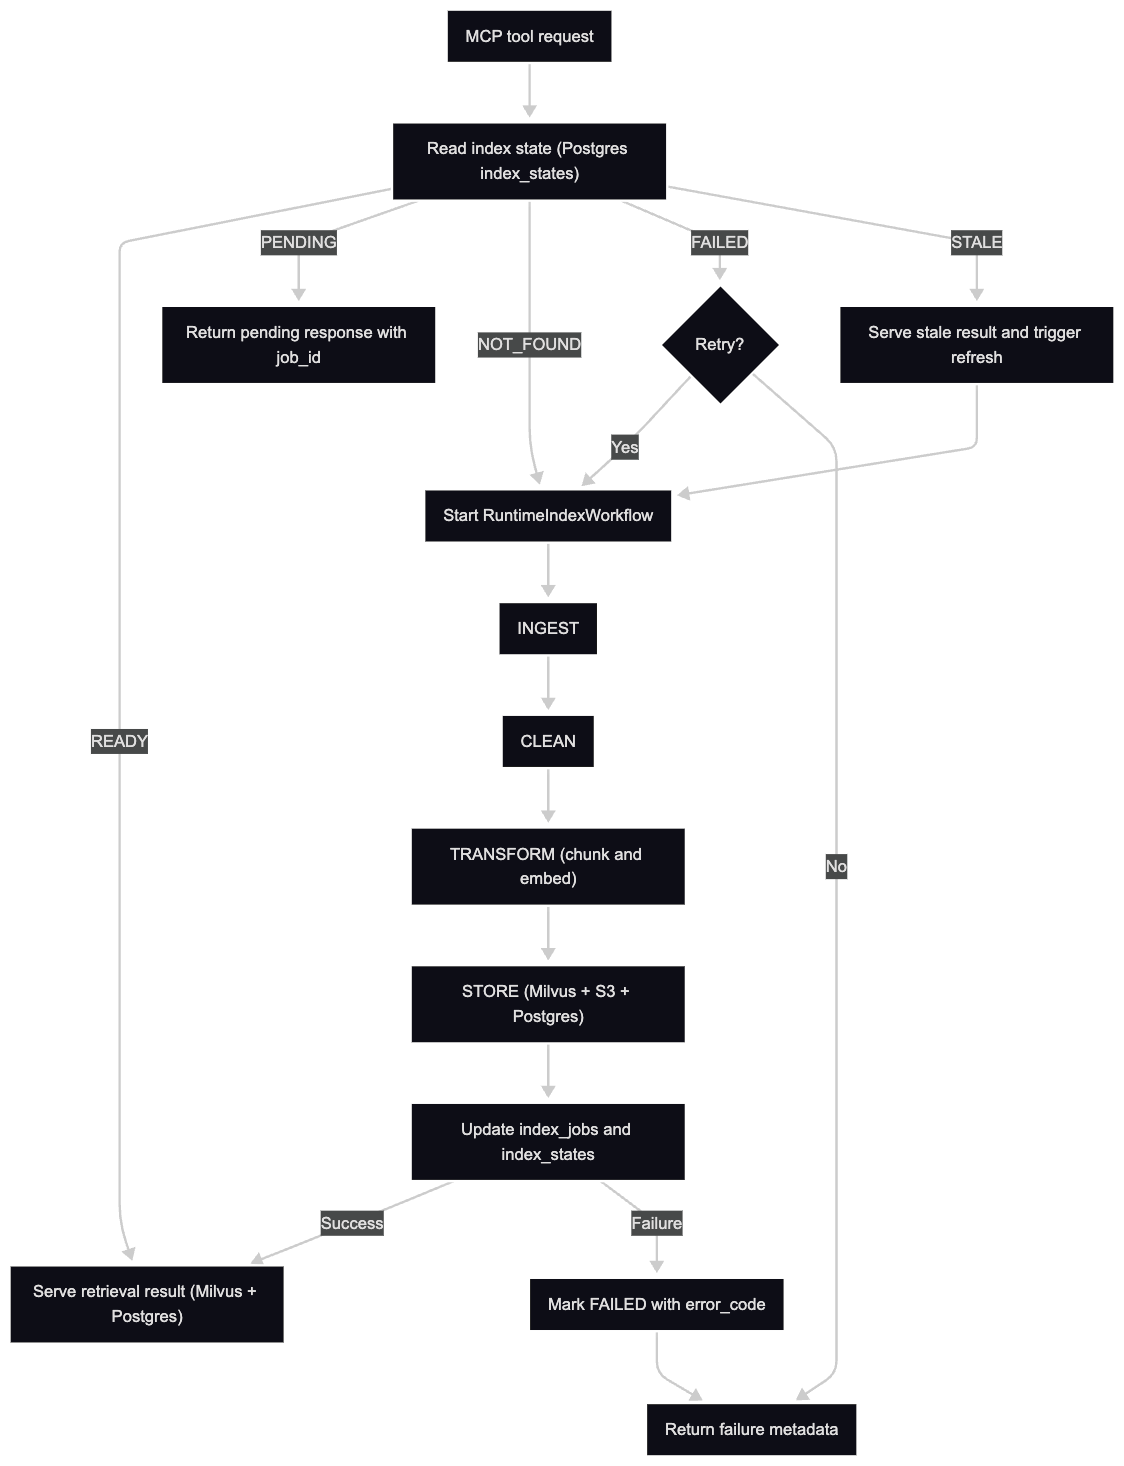
\includegraphics[width=\linewidth]{images/RuntimeIndexWorkflow.png}
  \caption{Runtime indexing workflow (\texttt{RuntimeIndexWorkflow}).}
  \label{fig:runtime-index-workflow}
\end{figure}

\begin{figure}[H]
  \centering
  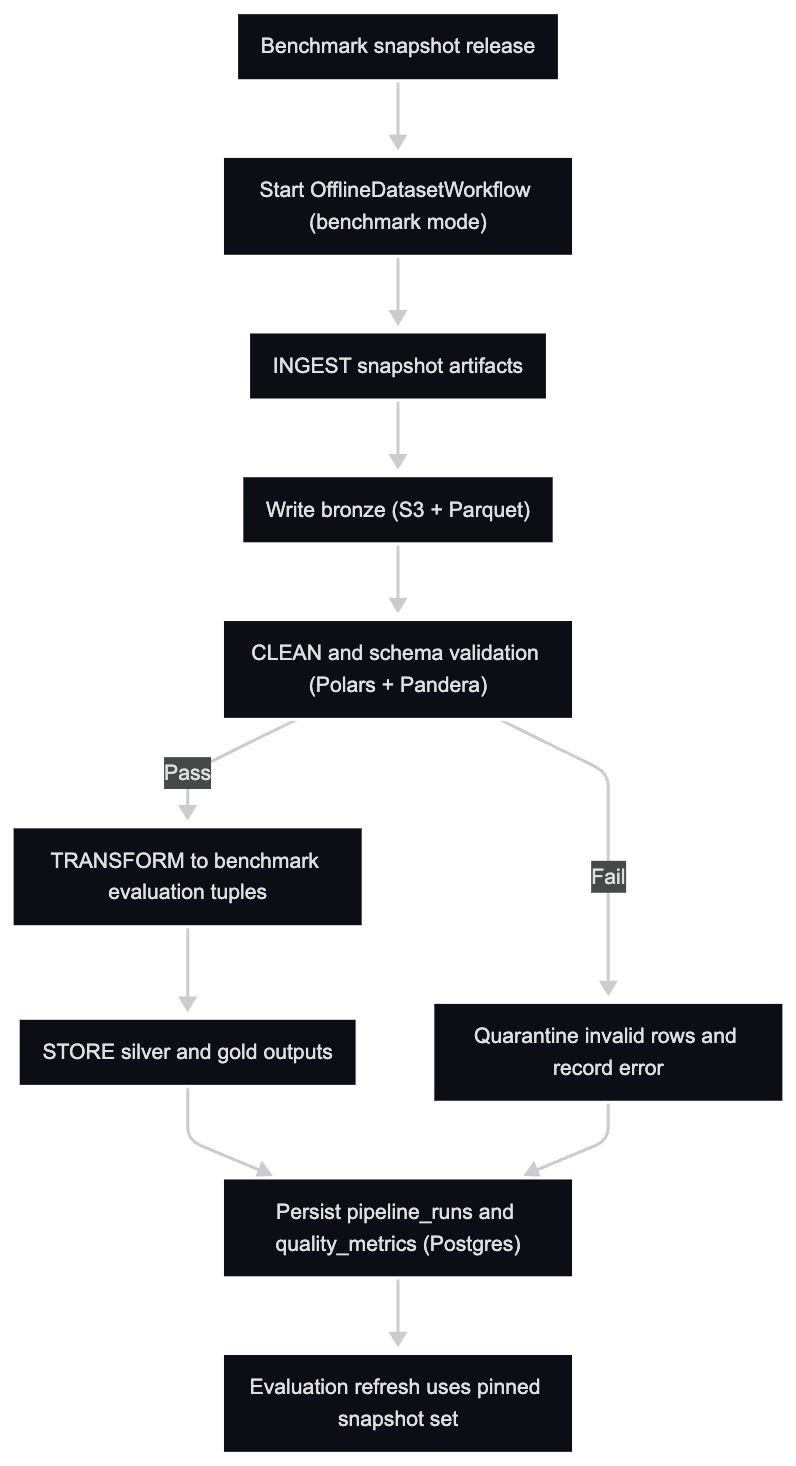
\includegraphics[width=0.72\linewidth]{images/OfflineDatasetWorkflow_benchmark.png}
  \caption{Offline benchmark snapshot workflow (\texttt{OfflineDatasetWorkflow}).}
  \label{fig:offline-benchmark-workflow}
\end{figure}

\begin{figure}[H]
  \centering
  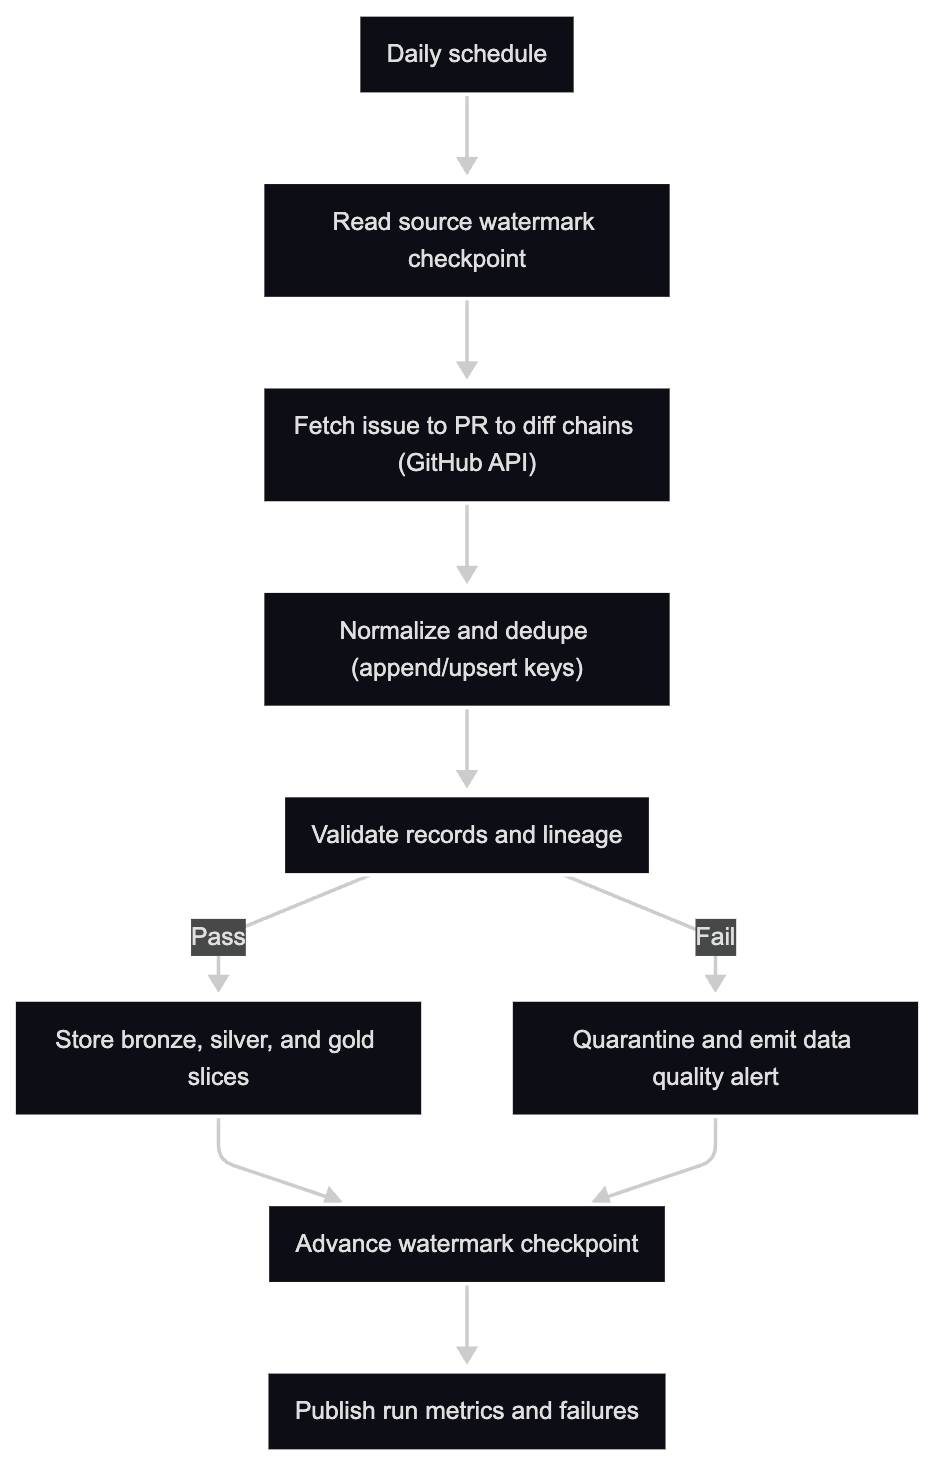
\includegraphics[width=0.72\linewidth]{images/OfflineDatasetWorkflow_rolling.png}
  \caption{Offline rolling scraped workflow (\texttt{OfflineDatasetWorkflow}).}
  \label{fig:offline-rolling-scraped-workflow}
\end{figure}

\begin{figure}[H]
  \centering
  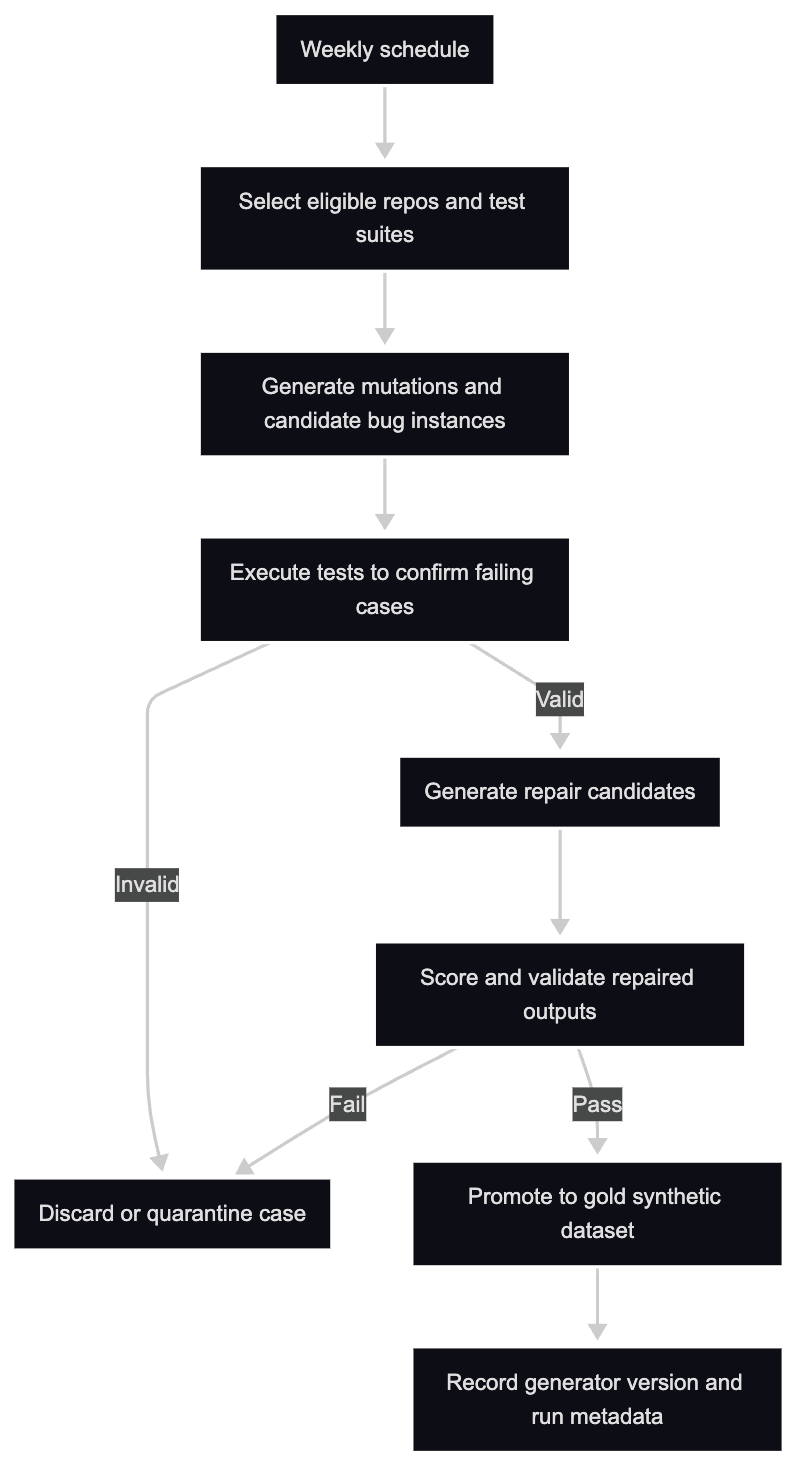
\includegraphics[width=0.72\linewidth]{images/OfflineDatasetWorkflow_synthetic.png}
  \caption{Offline synthetic refresh workflow (\texttt{OfflineDatasetWorkflow}).}
  \label{fig:offline-synthetic-refresh-workflow}
\end{figure}

\begin{figure}[H]
  \centering
  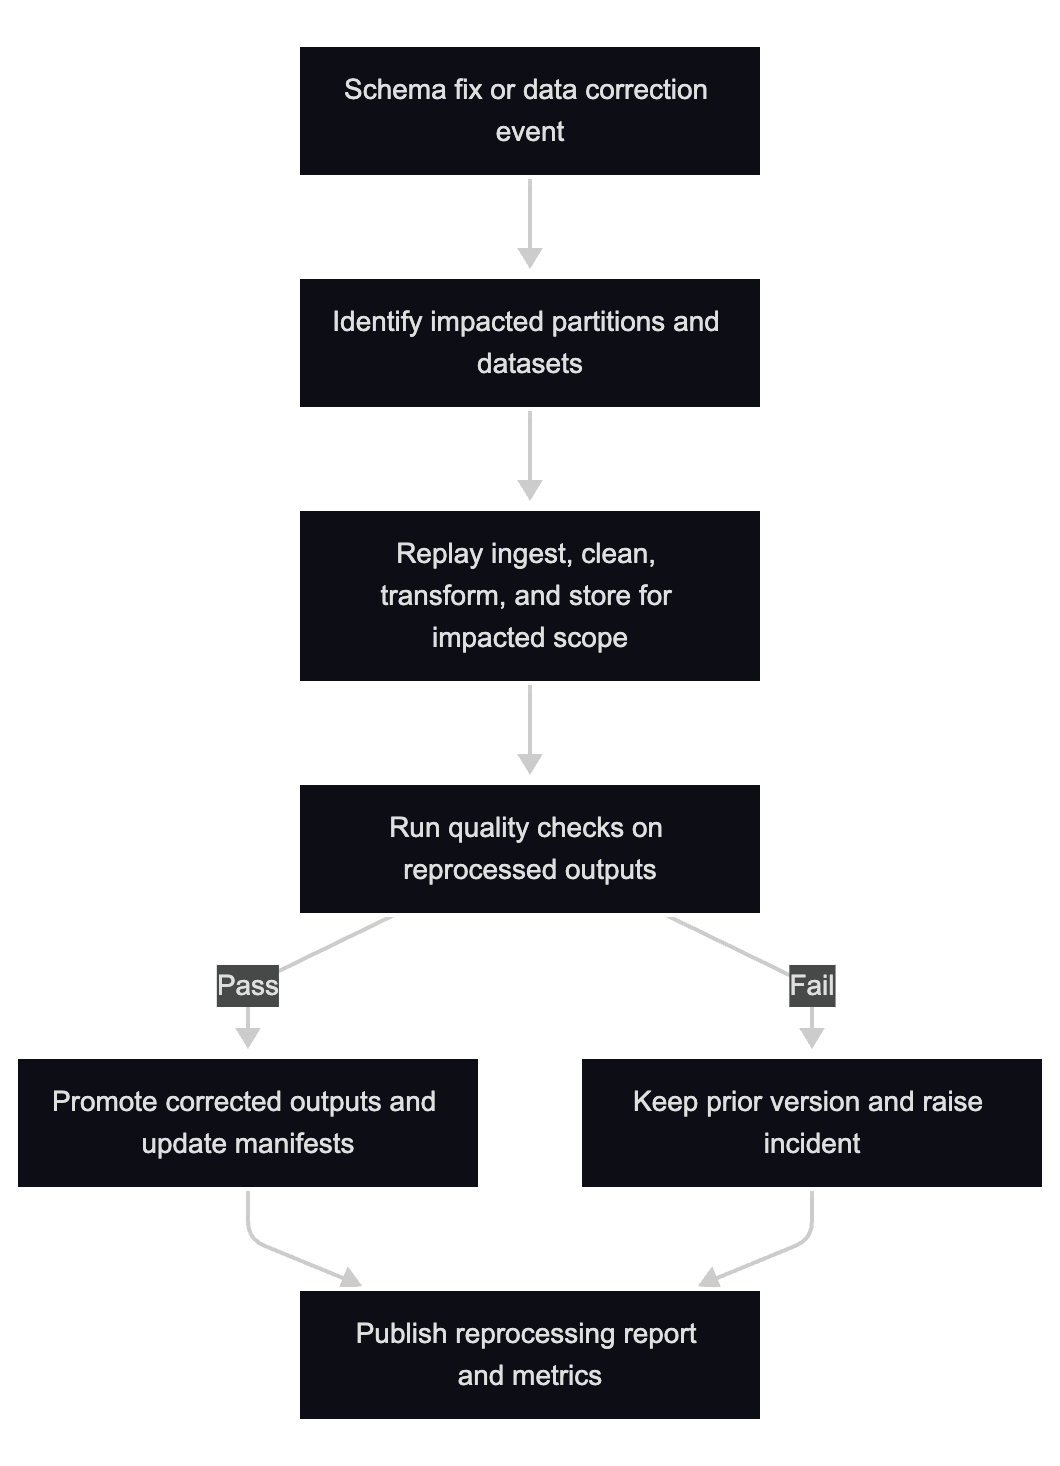
\includegraphics[width=0.72\linewidth]{images/OfflineDatasetWorkflow_reprocessing.png}
  \caption{Offline targeted reprocessing workflow (\texttt{OfflineDatasetWorkflow}).}
  \label{fig:offline-targeted-reprocessing-workflow}
\end{figure}

\begin{figure}[H]
  \centering
  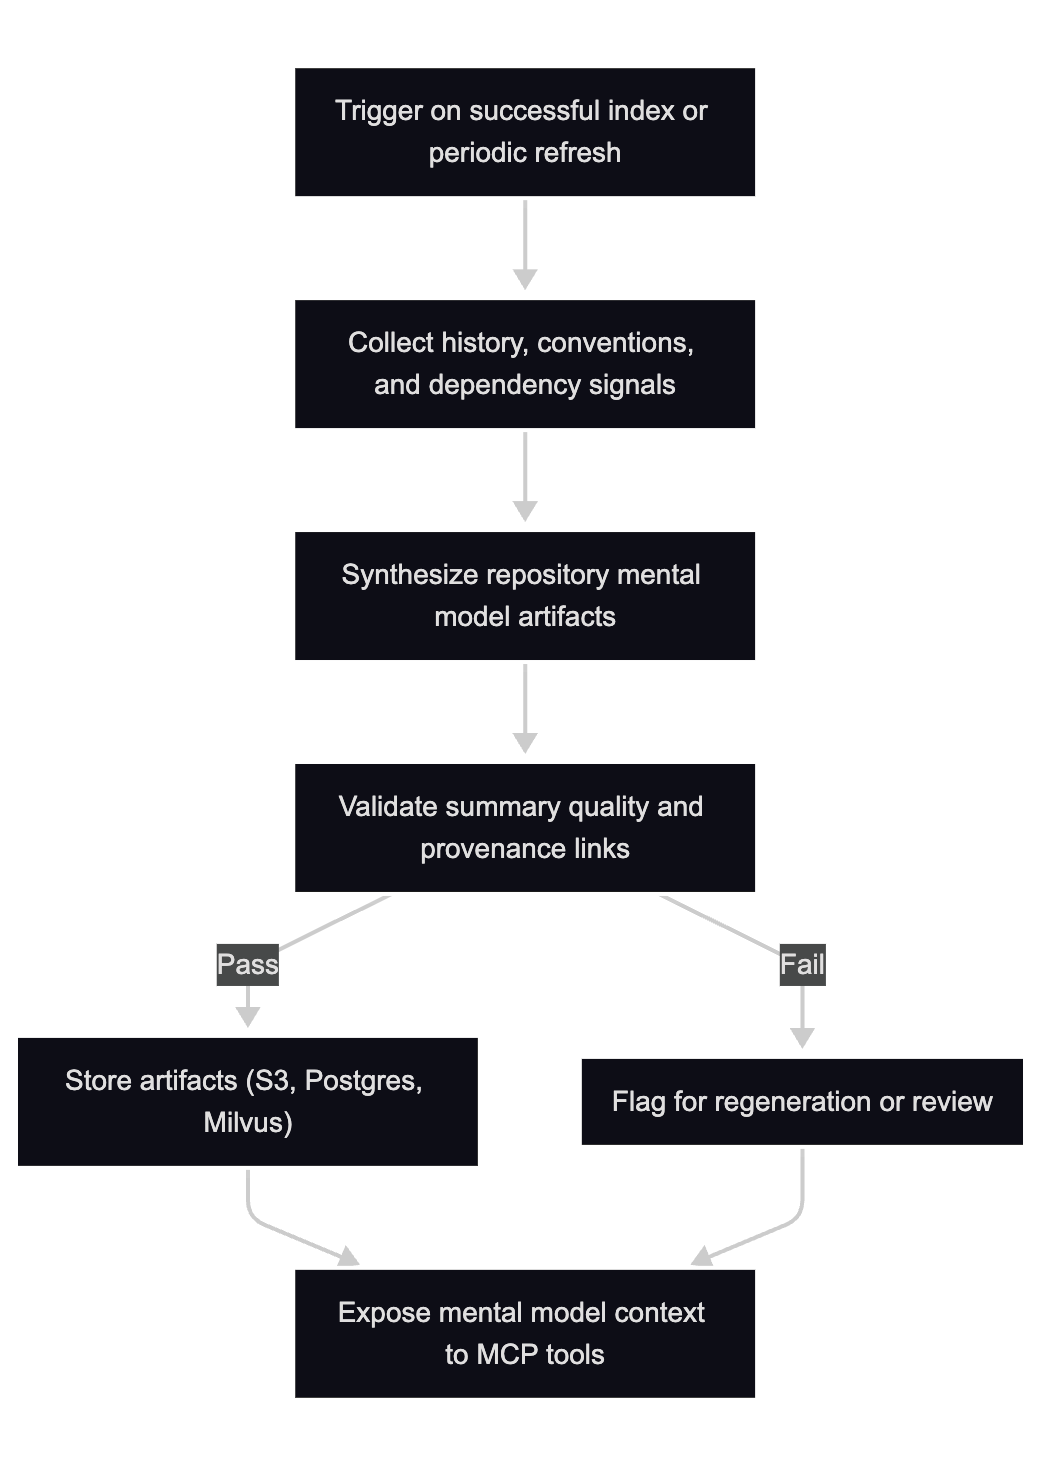
\includegraphics[width=0.72\linewidth]{images/MentalModelWorkflow.png}
  \caption{Mental model workflow (\texttt{MentalModelWorkflow}).}
  \label{fig:mental-model-workflow}
\end{figure}

% ================================================================================================
\subsection{Future Roadmap}

The first iteration established the end-to-end architecture, canonical schemas, and Temporal workflow structure, and it delivered a working online runtime-indexing pipeline plus benchmark snapshot ingestion for offline evaluation. The next iteration will focus on:

\begin{enumerate}
    \item Add a rolling scraped offline pipeline for incremental issue to PR to diff ingestion. This workflow will ingest new chains on a recurring cadence using append/upsert semantics keyed by stable source identifiers, rather than full rebuilds. The first implementation will focus on deterministic dedupe, watermark-based progress tracking, and run-level observability so ingestion can be resumed safely after failures.
    \item Add a synthetic offline pipeline for mutation-repair dataset refresh. This pipeline will generate controlled failing/repair examples on selected repositories with reliable test suites, then promote only validated outputs into gold datasets. Generator configuration, model version, and scoring settings will be versioned so synthetic data remains reproducible and comparable across runs.
    \item Expand offline schemas with high-confidence context-label attribution (\texttt{missing\_context}). The next schema revision will introduce explicit context-label tables and lineage links back to source artifacts and transforms. Initial labels will be weakly supervised and then calibrated through sampled review so downstream ranking/evaluation can account for label confidence.
    \item Train and integrate a learned retrieval-ranking layer over gold datasets. We will start with an offline training/evaluation loop that compares learned reranking against current retrieval baselines on fail-to-pass and regression metrics. Once stable, the ranker will be introduced behind configuration flags so rollout can be incremental and reversible.
\end{enumerate}


% ================================================================================================
%
%
%
%
%
% ================================================================================================

\section{IaC Implementation}

% Implement your pipeline infrastructure using code. You may choose any IaC framework, but your deployments should be straightforward and maintainable. For infrastructure components without existing modules:
% • Create your own modules when possible (e.g., creating a Terraform module instead of using scripts)
% • If using scripts, provide clear justification for this choice
% 4.1 Marking criteria:
% • Code clarity and organization
% • Infrastructure completeness
% • Alignment with parts 1,2,3
% • Implementation of multiple environments

% ================================================================================================
%
%
%
%
%
% ================================================================================================

% \section{Disaster Recovery Demonstration}

% Disaster has struck! Record a screen capture of your team deleting your production environment and your IaaC to restore it. Marks will be given on the completeness of the deletion restoration and clarity of the process/code.

% Demo should include:
% • Data processing services or deployed applications • Database systems and their data
% • Configuration settings
% • Access controls and security settings
% • Verification of system functionality 



% ================================================================================================
%
%
%
%
%
% ================================================================================================
\newpage
\appendix
\section*{Appendix}
\section{Aspirational Datasets: Schema Type Definitions}
\label{app:typedefs}

\subsection{Dataset 1: Context-Attributed Agent Failures}

\begin{tcolorbox}[title=AgentAttempt]
\footnotesize
\begin{tabularx}{\linewidth}{@{} l l Y @{}}
\toprule
\textbf{Field} & \textbf{Type} & \\
\midrule
diff & \texttt{Diff} & incorrect patch \\
files\_viewed & \texttt{[str]} & files inspected \\
searches\_performed & \texttt{[str]} & issued queries \\
\bottomrule
\end{tabularx}
\end{tcolorbox}

\begin{tcolorbox}[title=FailureSignal]
\footnotesize
\begin{tabularx}{\linewidth}{@{} l l Y @{}}
\toprule
\textbf{Field} & \textbf{Type} & \\
\midrule
type & \texttt{enum} & test\_failure $\mid$ type\_error $\mid$ runtime\_error $\mid$ semantic\_bug $\mid$ convention\_violation \\
message & \texttt{str} & diagnostic message \\
affected\_locations & \texttt{[\{file,line\}]} & manifestation points \\
\bottomrule
\end{tabularx}
\end{tcolorbox}

\begin{tcolorbox}[title=MissingContext]
\footnotesize
\begin{tabularx}{\linewidth}{@{} l l Y @{}}
\toprule
\textbf{Field} & \textbf{Type} & \\
\midrule
source & \texttt{enum} & same\_repo $\mid$ dependency $\mid$ documentation $\mid$ history \\
file & \texttt{str} & path / URL / commit \\
span & \texttt{(start,end)} & line range \\
content & \texttt{str} & contextual excerpt \\
context\_type & \texttt{enum} & contract $\mid$ caller $\mid$ type\_def $\mid$ invariant $\mid$ convention $\mid$ rationale $\mid$ config $\mid$ doc \\
explanation & \texttt{str} & why required \\
\bottomrule
\end{tabularx}
\end{tcolorbox}

% ================================================================================================
\subsection{Dataset 2: Interface Contracts and Cross-Boundary
Specifications}

\begin{tcolorbox}[title=Contract]
\footnotesize
\begin{tabularx}{\linewidth}{@{} l l Y @{}}
\toprule
\textbf{Field} & \textbf{Type} & \\
\midrule
signature & \texttt{str} & type signature / prototype \\
preconditions & \texttt{[str]} & required inputs \\
postconditions & \texttt{[str]} & guarantees on return \\
invariants & \texttt{[str]} & preserved properties \\
implicit & \texttt{[str]} & unwritten assumptions \\
source\_of\_truth & \texttt{enum} & type\_system $\mid$ docstring $\mid$ test\_assertion $\mid$ usage\_pattern $\mid$ unwritten \\
\bottomrule
\end{tabularx}
\end{tcolorbox}

\begin{tcolorbox}[title=Consumer]
\footnotesize
\begin{tabularx}{\linewidth}{@{} l l Y @{}}
\toprule
\textbf{Field} & \textbf{Type} & \\
\midrule
location & \texttt{\{repo,file,span\}} & call site \\
assumption\_relied\_on & \texttt{str} & contract dependency \\
\bottomrule
\end{tabularx}
\end{tcolorbox}

\begin{tcolorbox}[title=KnownViolation]
\footnotesize
\begin{tabularx}{\linewidth}{@{} l l Y @{}}
\toprule
\textbf{Field} & \textbf{Type} & \\
\midrule
diff & \texttt{Diff} & violating change \\
which\_contract\_broken & \texttt{str} & violated clause \\
failure\_mode & \texttt{str} & manifestation type \\
\bottomrule
\end{tabularx}
\end{tcolorbox}

% ================================================================================================
\subsection{Dataset 3: Downstream Impact Chains}

\begin{tcolorbox}[title=CausalNode]
\footnotesize
\begin{tabularx}{\linewidth}{@{} l l Y @{}}
\toprule
\textbf{Field} & \textbf{Type} & \\
\midrule
node & \texttt{\{file,function\}} & intermediate location \\
relationship & \texttt{enum} & calls $\mid$ inherits $\mid$ imports $\mid$ configures $\mid$ instantiates $\mid$ overrides \\
what\_propagates & \texttt{str} & propagated change (e.g.\ return type, side effect) \\
\bottomrule
\end{tabularx}
\end{tcolorbox}

% ================================================================================================
\subsection{Dataset 4: Architectural Conventions and Project Norms}

\begin{tcolorbox}[title=Convention]
\footnotesize
\begin{tabularx}{\linewidth}{@{} l l Y @{}}
\toprule
\textbf{Field} & \textbf{Type} & \\
\midrule
description & \texttt{str} & informal rule \\
category & \texttt{enum} & structural $\mid$ naming $\mid$ error\_handling $\mid$ concurrency $\mid$ security $\mid$ testing $\mid$ other \\
evidence & \texttt{[Evidence]} & pattern-establishing locations \\
codified\_in & \texttt{str $\mid$ null} & lint / ADR / style guide \\
\bottomrule
\end{tabularx}
\end{tcolorbox}

\begin{tcolorbox}[title=Evidence]
\footnotesize
\begin{tabularx}{\linewidth}{@{} l l Y @{}}
\toprule
\textbf{Field} & \textbf{Type} & \\
\midrule
file & \texttt{str} & file path \\
span & \texttt{(start,end)} & line range \\
\bottomrule
\end{tabularx}
\end{tcolorbox}

\begin{tcolorbox}[title=Violation]
\footnotesize
\begin{tabularx}{\linewidth}{@{} l l Y @{}}
\toprule
\textbf{Field} & \textbf{Type} & \\
\midrule
diff & \texttt{Diff} & violating change \\
what\_was\_violated & \texttt{str} & broken rule \\
corrected\_diff & \texttt{Diff} & fix \\
detection\_signal & \texttt{enum} & test\_failure $\mid$ review\_comment $\mid$ lint\_error $\mid$ silent\_bug \\
\bottomrule
\end{tabularx}
\end{tcolorbox}

% ================================================================================================
\subsection{Dataset 5: Design Rationale and Temporal Context}

\begin{tcolorbox}[title=HistoryEntry]
\footnotesize
\begin{tabularx}{\linewidth}{@{} l l Y @{}}
\toprule
\textbf{Field} & \textbf{Type} & \\
\midrule
commit & \texttt{sha} & commit id \\
timestamp & \texttt{datetime} & commit time \\
author & \texttt{str} & author \\
diff & \texttt{Diff} & change introduced \\
message & \texttt{str} & commit message \\
linked\_issue & \texttt{str $\mid$ null} & issue reference \\
\bottomrule
\end{tabularx}
\end{tcolorbox}

\begin{tcolorbox}[title=Rationale]
\footnotesize
\begin{tabularx}{\linewidth}{@{} l l Y @{}}
\toprule
\textbf{Field} & \textbf{Type} & \\
\midrule
summary & \texttt{str} & reason for current design \\
constraints & \texttt{[str]} & limiting factors \\
still\_relevant & \texttt{bool} & validity flag \\
invalidated\_by & \texttt{str $\mid$ null} & superseding event \\
\bottomrule
\end{tabularx}
\end{tcolorbox}

\begin{tcolorbox}[title=NaiveRefactor]
\footnotesize
\begin{tabularx}{\linewidth}{@{} l l Y @{}}
\toprule
\textbf{Field} & \textbf{Type} & \\
\midrule
diff & \texttt{Diff} & proposed change \\
why\_incorrect & \texttt{str} & breaking reason \\
failure\_signal & \texttt{str} & manifestation \\
\bottomrule
\end{tabularx}
\end{tcolorbox}

% ================================================================================================
\subsection{Dataset 6: Cross-Repository Dependency Context}

\begin{tcolorbox}[title=RequiredContext]
\footnotesize
\begin{tabularx}{\linewidth}{@{} l l Y @{}}
\toprule
\textbf{Field} & \textbf{Type} & \\
\midrule
source\_type & \texttt{enum} & source\_code $\mid$ docstring $\mid$ changelog $\mid$ migration\_guide $\mid$ issue\_thread $\mid$ example \\
location & \texttt{str} & path / URL \\
content & \texttt{str} & relevant excerpt \\
relevance & \texttt{str} & why it matters \\
\bottomrule
\end{tabularx}
\end{tcolorbox}

\begin{tcolorbox}[title=VersionSensitivity]
\footnotesize
\begin{tabularx}{\linewidth}{@{} l l Y @{}}
\toprule
\textbf{Field} & \textbf{Type} & \\
\midrule
valid\_for & \texttt{version\_range} & safe versions \\
breaks\_at & \texttt{version $\mid$ null} & breaking version \\
breaking\_change & \texttt{str $\mid$ null} & behavioral change \\
\bottomrule
\end{tabularx}
\end{tcolorbox}

\begin{tcolorbox}[title=MisuseExample]
\footnotesize
\begin{tabularx}{\linewidth}{@{} l l Y @{}}
\toprule
\textbf{Field} & \textbf{Type} & \\
\midrule
diff & \texttt{Diff} & incorrect change \\
assumption\_violated & \texttt{str} & broken assumption \\
failure\_signal & \texttt{str} & manifestation \\
\bottomrule
\end{tabularx}
\end{tcolorbox}

% ================================================================================================
\end{document}
